%----------------------------------------------------------------------------------------
%	PACKAGES AND THEMES
%----------------------------------------------------------------------------------------
\documentclass[aspectratio=169]{beamer}
%\usetheme{Simple}

\usepackage{listings}
\usepackage{lmodern}
 \setbeamercovered{transparent}
 \usetheme[width=4\baselineskip,hideothersubsections]{Berkeley}

 \setbeamerfont{section in sidebar}{size=\scriptsize}
 \setbeamerfont{subsection in sidebar}{size=\tiny}

 \usepackage{tikz}
 \usetikzlibrary{external}
 

 \usepackage{braket}

% \usepackage{graphicx} % Allows including images

% \usepackage{subcaption} % Subfigure environment 
% \usepackage{gensymb}

 \usepackage{amsmath} % Mathematical symbols
\usepackage{amssymb} % Symbols

% \usepackage{caption}% Captions onder figuur gecentreerd
% %\usepackage[toc,page]{appendix}
% \usepackage{subcaption} % Subfigure environment 
% \usepackage{float}

 \usepackage{etoolbox} %for if empty functionality
 \usepackage{ifthen}

% %break long urls at a - and not only at . or /
 \usepackage{hyperref}

% \usepackage{verbatim}
% \usepackage{siunitx} % Elegant eenheden zetten
% \usepackage[version=3]{mhchem} % ingeven van chemische fomules
\usepackage{cleveref} % Paragraaf tekens
% \usepackage{longtable}
% %\usepackage{lscape}
% \usepackage[T1]{fontenc}
 \usepackage{amsfonts}
 \usepackage{mathtools}
% \usepackage{grffile}%double dot in figure name
% \usepackage{lipsum}
% \usepackage{siunitx}
% \usepackage{xcolor}
% \usepackage{sectsty}
 \usepackage{booktabs}
 \usepackage{physics}
% \usepackage{leftidx}
 \usepackage[utf8]{inputenc}
% \usepackage{gensymb} % /textdegree


%----------------------------------------------------------------------------------------
%	TITLE PAGE
%----------------------------------------------------------------------------------------

% The title
\title[]{PEPO cluster expansion of Tensor Exponential  }
\subtitle{Subtitle}

\author[] {David Devoogdt}
\institute[UGent] % Your institution may be shorthand to save space
{
    % Your institution for the title page
    Faculty of Engineering and Architecture \\
    Ghent University 
    \vskip 3pt
}
\date{\today} % Date, can be changed to a custom date


%\def\temp{#1}\ifx\temp\empty
%  <EMPTY>%
%\else
%  <NON EMPTY>%
%\fi

\newcommand{\combineTikz}[3]{
    \begin{tikzpicture}[baseline={0-0.5*height("$=$")}]
        \node (AA) at (0,0)  { #1   };
        \node (AB) at ( {#3} ,0)  {  #2  };
    \end{tikzpicture}
}

%\newcommand{\mpo}[6]  {\tikzexternalenable { \begin{tikzpicture}[baseline={0-0.5*height("$=$")}]
\newcommand{\mpo}[6]  { \begin{tikzpicture}[baseline={0-0.5*height("$=$")}]

        %\def \NNodes {#1}
        %\def \NodeName {#2}          
        %\def \NodeName {#2}          
        %\def \NodeName {#2}          
        %\def \NodeName {#2}          
        %\def \NodeName {#2}          
        %\def \NameUp   {#3} 
        %\def \NameUp   {#3} 
        %\def \NameUp   {#3} 
        %\def \NameUp   {#3} 
        %\def \NameUp   {#3} 
        %\def \NameDown  {#4}	
        %\def \NameDown  {#4}	
        %\def \NameDown  {#4}	
        %\def \NameDown  {#4}	
        %\def \NameDown  {#4}	

        \def \legLength {0.7}
        \def \radius {0.3}

        \pgfmathsetmacro{\step}{2*\radius+\legLength}
        \pgfmathsetmacro{\legpos}{\radius+\legLength}

        \pgfmathsetmacro{\Nmax}{#1-1}

        \foreach \N in {0,..., \Nmax }{
                \pgfmathsetmacro{\p}{\N*\step}

                % up and down labels
                \def\temp{#3}\ifx\temp\empty
                    \def \labelUp {}
                \else
                    \pgfmathsetmacro{\labelUp}{  {#3}[\N]  }
                \fi

                \def\tempp{#4}\ifx\tempp\empty
                    \def \labeldown {}
                \else
                    \pgfmathsetmacro{\labeldown}{  {#4}[\N]  }
                \fi

                \def\aab{#5}\ifx\aab\empty
                    \def \dotssite {0}
                \else
                    \pgfmathsetmacro{\dotssite}{  {#5}[\N]  }
                \fi

                \ifthenelse{\dotssite = 0}{

                    \def\aac{#6}\ifx\aac\empty
                        \def \nname {O}
                    \else
                        \pgfmathsetmacro{\nname}{  {#6}[\N]  }
                    \fi

                    \node[circle,draw, radius=\radius] (O\N) at (\p,0) {\nname};

                    \ifthenelse{ \equal{\labelUp}{-}  }{
                    }{
                        \node[] (Ou\N) at (\p, \legpos ) { \labelUp };
                        \draw (O\N) -- (Ou\N);
                    }

                    \ifthenelse{ \equal{\labeldown}{-}  }{
                    }{
                        \node[] (Od\N) at (\p,-\legpos) {\labeldown};
                        \draw (O\N) -- (Od\N);
                    }

                }{
                    \node[circle] (O\N) at (\p,0) { $\cdots$ };
                }

            }

        \ifthenelse{  #1  =1  }{}{
            \foreach \N in {1,...,\Nmax }{
                    \pgfmathsetmacro{\M}{\N-1}
                    \pgfmathsetmacro{\label}{ {#2}[\N]  }
                    %\pgfmathsetmacro{\label}{ 5}

                    \draw (O\M) --  node[above]  {\label} (O\N);
                }
        }

        \pgfmathsetmacro{\labelo}{ {#2}[0]}
        \pgfmathsetmacro{\labeli}{  {#2}[\Nmax+1]}

        \ifthenelse{ \equal{\labelo}{Tr}  }{

            \pgfmathsetmacro{\endpos}{\step*\Nmax+\radius}

            \draw plot [smooth ]  coordinates { (-\radius,0)    (-\radius, -0.45 )  (\endpos, -0.45)   (O\Nmax)   } ;
        }{
            \ifthenelse{ \equal{\labelo}{-}  }{
            }{
                \pgfmathsetmacro{\endpos}{\step*\Nmax+\legpos}

                \node (N0) at (-\legpos,0) {};
                \node (Ne) at (\endpos,0) {};

                \draw (N0) -- node[above] {\labelo} (O0);

                \draw (Ne) -- node[above] {\labeli}  (O\Nmax);
            }
        }
        %\draw (O0) --  node[above] {1} (O1);
        %\end{tikzpicture}} \tikzexternaldisable}
    \end{tikzpicture}}

%\newcommand{\expH}[5]{\tikzexternalenable { \begin{tikzpicture}[baseline={0-0.5*height("$=$")}]
\newcommand{\expH}[5]{\begin{tikzpicture}[baseline={0-0.5*height("$=$")}]
        \def \NNodes {#1};

        \def\aaa{#2}\ifx\aaa\empty
            \def \text { $e^{-\beta \hat{H}_{\NNodes} }$ }
        \else
            \def \text {#2}
        \fi

        \pgfmathwidth{ "\text" }
        \def \textwidth { \pgfmathresult }

        %\pgfmathsetmacro{\text}{width(\text)}

        \def \legLength {0.6}
        \def \radius {0.3} %fix to fit text inside for size 1
        \def \boxHeight {0.4};

        \pgfmathsetmacro{\step}{2*\radius+\legLength}
        \pgfmathsetmacro{\legpos}{\radius+\legLength}
        \pgfmathsetmacro{\dotpos}{\boxHeight+\legLength/2}

        \pgfmathsetmacro{\Nmax}{\NNodes -1}

        \pgfmathsetmacro{\boxsize}{ max ( \textwidth/1cm , \step*\Nmax )   + \radius}

        %\pgfmathsetmacro{\boxsize}{ 5  )}
        %\pgfmathsetlength{\boxsize}{ max( \textwidth,  \boxsize1  )}

        %            \ifthenelse{#1=1}{
        %                \def \left {-0.6}
        %                \def \right {0.6}
        %            }{
        \def \left {-\radius}
        \def \right {\boxsize}
        %            }

        \draw (\left,- \boxHeight ) rectangle (\right, \boxHeight ) [add reference =H] ;

        \node  at (H center) { \text };

        \foreach \N in {0,..., \Nmax }{
                \pgfmathsetmacro{\p}{\N*\step}

                % up and down labels
                \def\temp{#3}\ifx\temp\empty
                    \def \labelUp {}
                \else
                    \pgfmathsetmacro{\labelUp}{  {#3}[\N]  }
                \fi

                \def\tempp{#4}\ifx\tempp\empty
                    \def \labeldown {}
                \else
                    \pgfmathsetmacro{\labeldown}{  {#4}[\N]  }
                \fi

                \node[] (O\N) at (\p,0) {};

                \ifthenelse{ \equal{\labelUp}{...}  }{
                    \node[] (Ou\N) at (\p, \dotpos ) {\labelUp};
                }{
                    \ifthenelse{ \equal{\labelUp}{-}  }{

                    }{
                        \node[] (Ou\N) at (\p, \legpos ) {\labelUp};
                        \draw (Ou\N) --  (Ou\N  |- H north);
                    }
                }

                \ifthenelse{ \equal{\labeldown}{...}  }{
                    \node[] (Od\N) at (\p,-\dotpos ) {\labeldown};
                }{
                    \ifthenelse{ \equal{\labeldown}{-}  }{

                    }{
                        \node[] (Od\N) at (\p,-\legpos) {\labeldown};
                        \draw (Od\N) --  (Od\N  |- H south);
                    }
                }
            }

        \def\tempt{#5}\ifx\tempt\empty

        \else
            \pgfmathsetmacro{\labelo}{ {#5}[0] }
            \pgfmathsetmacro{\labeli}{  {#5}[1] }

            \pgfmathsetmacro{\leftleg}{  \left - \legLength }
            \pgfmathsetmacro{\rightleg}{  \right + \legLength }

            \node (N0) at (\leftleg,0) {\labelo};
            \draw (N0) -- ( N0  -| H west);

            \node (Ne) at (\rightleg,0) {\labeli};
            \draw (Ne) --  ( Ne  -| H east);
        \fi

        %        \end{tikzpicture}} \tikzexternaldisable }
    \end{tikzpicture} }

%\newcommand{\mpob}[6]  {\tikzexternalenable { \begin{tikzpicture}[baseline={0-0.5*height("$=$")},scale=0.8]
\newcommand{\mpob}[6]  {\begin{tikzpicture}[baseline={0-0.5*height("$=$")},scale=0.8]

        %\def \NNodes {#1}
        %\def \NodeName {#2}          
        %\def \NodeName {#2}          
        %\def \NodeName {#2}          
        %\def \NodeName {#2}          
        %\def \NodeName {#2}          
        %\def \NameUp   {#3} 
        %\def \NameUp   {#3} 
        %\def \NameUp   {#3} 
        %\def \NameUp   {#3} 
        %\def \NameUp   {#3} 
        %\def \NameDown  {#4}	
        %\def \NameDown  {#4}	
        %\def \NameDown  {#4}	
        %\def \NameDown  {#4}	
        %\def \NameDown  {#4}	

        \def \legLength {1.0}
        \def \radius {0.1}

        \pgfmathsetmacro{\step}{2*\radius+\legLength}
        \pgfmathsetmacro{\legpos}{\radius+\legLength}

        \pgfmathsetmacro{\Nmax}{#1-1}

        \foreach \N in {0,..., \Nmax }{
                \pgfmathsetmacro{\p}{\N*\step}

                % up and down labels
                \def\temp{#3}\ifx\temp\empty
                    \def \labelUp {}
                \else
                    \pgfmathsetmacro{\labelUp}{  {#3}[\N]  }
                \fi

                \def\tempp{#4}\ifx\tempp\empty
                    \def \labeldown {}
                \else
                    \pgfmathsetmacro{\labeldown}{  {#4}[\N]  }
                \fi

                \def\aab{#5}\ifx\aab\empty
                    \def \dotssite {0}
                \else
                    \pgfmathsetmacro{\dotssite}{  {#5}[\N]  }
                \fi

                \def\aac{#6}\ifx\aac\empty
                    \def \nname { "O" }
                \else
                    \pgfmathsetmacro{\nname}{  {#6}[\N]  }
                \fi

                %\node[] (O\N) at (\p,0) {\nname};
                \node[circle,draw, radius=\radius] (O\N) at (\p,0) {\nname};

            }

        \ifthenelse{  #1  =1  }{}{
            \foreach \N in {1,...,\Nmax }{
                    \pgfmathsetmacro{\M}{\N-1}
                    \pgfmathsetmacro{\label}{ {#2}[\N]  }
                    %\pgfmathsetmacro{\label}{ 5}

                    \draw (O\M) --  node[above]  {\label} (O\N);
                }
        }

        % \pgfmathsetmacro{\labelo}{ {#2}[0]}
        % \pgfmathsetmacro{\labeli}{  {#2}[\Nmax+1]}

        % \node (N0) at (-\legpos,0) {};
        % \draw (N0) -- node[above] {\labelo} (O0);

        % \pgfmathsetmacro{\endpos}{\step*\Nmax+\legpos}

        % \node (Ne) at (\endpos,0) {};
        % \draw (Ne) -- node[above] {\labeli} (O\Nmax);

        %\draw (O0) --  node[above] {1} (O1);

        % \end{tikzpicture}} \tikzexternaldisable}

    \end{tikzpicture}}

% \newcommand{\pepob}[5]  { \tikzexternalenable {\begin{tikzpicture}[baseline={0-0.5*height("$=$")},scale=0.8]
% \newcommand{\pepob}[5]  { \begin{tikzpicture}[baseline={0-0.5*height("$=$")},scale=1,
\newcommand{\pepob}[5]  { \begin{tikzpicture}[
            baseline={([yshift= -2ex ]current bounding box.north)},
            %baseline={0-0.5*height("$=$")},
            scale=1,
            Al/.style = {regular polygon, regular polygon sides=3,
                    draw, fill=white, text width=0.1,
                    inner sep=1mm, outer sep=0mm,
                    shape border rotate=-90},
            Ar/.style = {regular polygon, regular polygon sides=3,
                    draw, fill=white, text width=0.1,
                    inner sep=1mm, outer sep=0mm,
                    shape border rotate=90},
            Acc/.style = {diamond, draw, inner sep=1mm},
            Ac/.style = {rectangle, draw, inner sep=2mm}]

        %\pgfmathsetmacro{\llegLength}{ 0.3 }

        \def \legLength { 0.8}
        \def \radius {0.1}

        %\pgfmathtruncatemacro{\llegLength} { 0.8 }
        %\pgfmathtruncatemacro{\radius} { 0.1 }

        %\pgfmathtruncatemacro{\legLength}{2* \llegLength}
        %\pgfmathtruncatemacro{\lstep}{\radius+ \llegLength}
        %\pgfmathtruncatemacro{\step}{2*\lstep}
        \pgfmathsetmacro{\step}{2*\radius+ \legLength}

        \pgfmathsetmacro{\legpos}{\radius+\legLength}

        \pgfmathsetmacro{\Nmax}{#1-1}
        \pgfmathsetmacro{\Mmax}{#2-1}

        % define positions of different O's

        \setcounter{a}{0}
        %\setcounter{a}{0}

        \foreach \N in {0,..., \Nmax }{

                %\pgfmathtruncatemacro{\a}{\thea}

                \pgfmathsetmacro{\p}{  (\N + \thea) *\step   }
                %\setcounter{b}{0}

                \foreach \M in {0,..., \Mmax }{

                        %\pgfmathsetmacro{\p}{ \pp + \theb *\step   }

                        \pgfmathsetmacro{\k}{   \M   *\step  }

                        \pgfmathtruncatemacro{\s}{\M*(\Nmax+1)+\N   }

                        \pgfmathsetmacro{\nname}{ ""  }

                        \def\aab{#5}\ifx\aab\empty
                            \def \so {0}
                        \else
                            \pgfmathsetmacro{\so}{  {#5}[\s]  }
                        \fi

                        \ifthenelse{\so = 0}{
                            \node[circle,draw, radius=\radius] (O\s) at (\p,\k) {\nname};
                        }

                        \ifthenelse{\so = 2}{
                            \node[draw, Al] (O\s) at (\p,\k) {\nname};
                        }

                        \ifthenelse{\so = 3}{
                            \node[draw, Ar] (O\s) at (\p,\k) {\nname};
                        }

                        \ifthenelse{\so = 4}{
                            \node[draw= none, inner sep=0, outer sep=0 , minimum size=0pt] (O\s) at (\p,\k) {\nname};
                        }

                        \ifthenelse{\so = 6}{
                            \node[draw, Acc] (O\s) at (\p,\k) {\nname};
                        }

                        \ifthenelse{\so = 7}{
                            \node[draw, Ac] (O\s) at (\p,\k) {\nname};
                        }

                        %Gl environment
                        \ifthenelse{\so = 5}{

                            \pgfmathsetmacro{\recl}{  \p + \step - 3*\radius  }
                            \pgfmathsetmacro{\recr}{  \p + \step + 3*\radius  }

                            \pgfmathsetmacro{\recu}{  \k + 2*\radius }
                            \pgfmathsetmacro{\recd}{  \k - \step -2*\radius  }

                            % \pgfmathsetmacro{\recl}{  \p  +\step   }
                            % \pgfmathsetmacro{\mw}{ 2*\radius }
                            % \pgfmathsetmacro{\mh}{ \step  }

                            % \pgfmathsetmacro{\recu}{  \k - \step /2 }

                            % \node[rectangle,
                            %     draw,
                            %     minimum height= 1,
                            %     anchor=center  ] (O\s) at (\recl,\recu) {Gl};

                            \draw  (\recl,\recu) rectangle node[  ] (O\s)  {Gl}   (\recr,\recd)     ;

                            %\draw node[fill, minimum width= 1  ,minimum height= 1 ] (O\s) at (\recl,\recu) {Gl};
                            \stepcounter{a}
                        }

                        \ifthenelse{\so = 8}{

                            \node[draw, Ar] (O\s) at (\p,\k) {\nname};

                            \pgfmathtruncatemacro{\t}{\M*(\Nmax+1)+\N +1  }

                            \pgfmathsetmacro{\recl}{  \p +\step  - 3*\radius  }
                            \pgfmathsetmacro{\recr}{  \p + \step+  3*\radius  }

                            \pgfmathsetmacro{\recu}{  \k + 2*\radius }
                            \pgfmathsetmacro{\recd}{  \k - \step -2*\radius  }

                            \draw  (\recl,\recu) rectangle node (O\t)  {Gr}   (\recr,\recd)     ;

                            \draw  (O\s) -- (   O\t.west   |-  O\s  ) ;
                            \stepcounter{a}
                        }

                        \ifthenelse{\so = 9}{

                            \node[draw, Ac] (O\s) at (\p,\k) {\nname};

                            \pgfmathtruncatemacro{\t}{\M*(\Nmax+1)+\N +1  }

                            \pgfmathsetmacro{\recl}{  \p +\step  - 3*\radius  }
                            \pgfmathsetmacro{\recr}{  \p + \step+  3*\radius  }

                            \pgfmathsetmacro{\recu}{  \k + 2*\radius }
                            \pgfmathsetmacro{\recd}{  \k - \step -2*\radius  }

                            \draw  (\recl,\recu) rectangle node (O\t)  {Gr}   (\recr,\recd)     ;

                            \draw  (O\s) -- (   O\t.west   |-  O\s  ) ;
                            \stepcounter{a}
                        }

                        \ifthenelse{\so = 10}{

                            \node[draw = none] (O\s) at (\p,\k) {\nname};

                            \pgfmathtruncatemacro{\t}{\M*(\Nmax+1)+\N +1  }

                            \pgfmathsetmacro{\recl}{  \p +\step  - 3*\radius  }
                            \pgfmathsetmacro{\recr}{  \p + \step+  3*\radius  }

                            \pgfmathsetmacro{\recu}{  \k + 2*\radius }
                            \pgfmathsetmacro{\recd}{  \k - \step -2*\radius  }

                            \draw  (\recl,\recu) rectangle node (O\t)  {Gr}   (\recr,\recd)     ;

                            \draw  (O\s) -- (   O\t.west   |-  O\s  ) ;
                            \stepcounter{a}
                        }

                        \ifthenelse{\so = 11}{

                            \node[draw , Acc] (O\s) at (\p,\k) {\nname};

                            \pgfmathtruncatemacro{\t}{\M*(\Nmax+1)+\N +1  }

                            \pgfmathsetmacro{\recl}{  \p +\step  - 3*\radius  }
                            \pgfmathsetmacro{\recr}{  \p + \step+  3*\radius  }

                            \pgfmathsetmacro{\recu}{  \k + 2*\radius }
                            \pgfmathsetmacro{\recd}{  \k - \step -2*\radius  }

                            \draw  (\recl,\recu) rectangle node (O\t)  {Gr}   (\recr,\recd)     ;

                            \draw  (O\s) -- (   O\t.west   |-  O\s  ) ;
                            \stepcounter{a}
                        }

                        \ifthenelse{\so = 12}{

                            \node[circle,draw, radius=\radius] (O\s) at (\p,\k) {\nname};

                            \pgfmathsetmacro{\pp}{   \p+\legLength/2 }
                            \pgfmathsetmacro{\pm}{   \p-\legLength/2  }

                            \pgfmathsetmacro{\kp}{   \k+\legLength/2  }
                            \pgfmathsetmacro{\km}{   \k-\legLength/2  }

                            \node (Op\s) at (\pp,\kp) {i};
                            \node (Om\s) at (\pm,\km) {j};

                            \draw (O\s.center)  --  (Op\s);
                            \draw  (Om\s) --  (O\s);
                        }

                        \ifthenelse{\so = 13}{

                            \node[draw= none] (O\s) at (\p,\k) { ... };
                        }

                        \ifthenelse{\so = 14}{

                            \node[circle,draw, radius=\radius] (O\s) at (\p,\k) {\nname};

                            \pgfmathsetmacro{\pp}{   \p+\legLength/2 }
                            \pgfmathsetmacro{\pm}{   \p-\legLength/2  }

                            \pgfmathsetmacro{\kp}{   \k+\legLength/2  }
                            \pgfmathsetmacro{\km}{   \k-\legLength/2  }

                            \node (Op\s) at (\pp,\kp) {};
                            \node (Om\s) at (\pm,\km) {};

                            \draw (O\s.center)  --  (Op\s);
                            \draw  (Om\s) --  (O\s);
                        }

                        \ifthenelse{\so = 15}{

                            \node[circle,draw, radius=\radius] (O\s) at (\p,\k) {\nname};

                            \pgfmathsetmacro{\pp}{   \p+\legLength/2 }

                            \pgfmathsetmacro{\kp}{   \k+\legLength/2  }

                            \node (Op\s) at (\pp,\kp) {};

                            \draw (O\s.center)  --  (Op\s);
                        }

                        \ifthenelse{\so = 16}{
                            \node[draw, Ac] (O\s) at (\p,\k) {B};
                        }

                        \ifthenelse{\so = 17}{
                            \node[circle,draw=none, radius=\radius] (O\s) at (\p,\k) {\nname};
                        }

                        \ifthenelse{\so = 18}{

                            \node[circle,draw=none, radius=\radius] (O\s) at (\p,\k) {\nname};

                            \pgfmathtruncatemacro{\t}{\M*(\Nmax+1)+\N +1  }

                            \pgfmathsetmacro{\recl}{  \p +\step  - 3*\radius  }
                            \pgfmathsetmacro{\recr}{  \p + \step+  3*\radius  }

                            \pgfmathsetmacro{\recu}{  \k + 2*\radius }
                            \pgfmathsetmacro{\recd}{  \k - \step -2*\radius  }

                            \draw  (\recl,\recu) rectangle node (O\t)  {Gr}   (\recr,\recd)     ;

                            \draw  (O\s) -- (   O\t.west   |-  O\s  ) ;
                            \stepcounter{a}
                        }

                        \ifthenelse{\so = 22}{
                            \node[draw,line width=0.6mm  ,Al] (O\s) at (\p,\k) {};
                        }

                        \ifthenelse{\so = 23}{
                            \node[draw,line width=0.6mm  ,Ar] (O\s) at (\p,\k) {};
                        }

                        \ifthenelse{\so = 25}{
                            \node[draw,line width=0.6mm ,Ac] (O\s) at (\p,\k) {};
                        }

                        \ifthenelse{\so = 24}{
                            \node[draw, Ac] (O\s) at (\p,\k) {Fl};
                        }

                        \ifthenelse{\so = 26}{
                            \node[draw, Ac] (O\s) at (\p,\k) {Fr};
                        }

                    }
            }

        %connect nodes horizontally with correct name
        \foreach \M in {0,..., \Mmax }{
                \foreach \N in {1,...,\Nmax}{

                        \pgfmathtruncatemacro{\s}{\M*(\Nmax+1)+\N   }

                        \pgfmathtruncatemacro{\t}{\M*(\Nmax+1)+\N  -1 }

                        \pgfmathtruncatemacro{\l}{\M*(\Nmax)+\N -1 }

                        %\pgfmathsetmacro{\label}{ {#2}[\N]  }
                        %\pgfmathsetmacro{\label}{ \l }
                        \pgfmathsetmacro{\label}{ {#3}[\l]  }

                        \def\aab{#5}\ifx\aab\empty
                            \def \so {0}
                        \else
                            \pgfmathsetmacro{\so}{  {#5}[\s]  }
                        \fi

                        \def\aab{#5}\ifx\aab\empty
                            \def \to {0}
                        \else
                            \pgfmathsetmacro{\to}{  {#5}[\t]  }
                        \fi

                        \ifthenelse{ \equal{\label}{Gl}  }{

                            \pgfmathtruncatemacro{\ogl}{ (\M+1)*(\Nmax+1)+\N -1 }

                            \draw (O\ogl.east   |- O\s  )  --  (O\s);

                            \draw (O\t)  --  ( O\ogl.west    |-  O\t  );

                        }{

                            \ifthenelse{ \equal{\label}{Gr}  }{

                                \pgfmathtruncatemacro{\ogl}{ (\M+1)*(\Nmax+1)+\N  }

                                \draw (O\t)  --  ( O\ogl.west    |-  O\t  );

                                \draw (O\ogl.east   |- O\s  )  --  (O\s);

                            }{

                                \ifthenelse{ \NOT  \so = 1  }{
                                    \ifthenelse{ \NOT  \to = 1}{
                                        \ifthenelse{ \equal{\label}{-} }{

                                        }
                                        {

                                            \draw ( O\t.east |- O\s )  --  node[above]  {\label} (O\s);
                                        }
                                    }
                                }
                            }

                        }

                    }
            }

        %connect nodes vertically with correct name
        \foreach \N in {0,...,\Nmax }{
                \foreach \M in {1,..., \Mmax }{

                        \pgfmathtruncatemacro{\s}{\M*(\Nmax+1)+\N   }

                        \pgfmathtruncatemacro{\t}{ (\M-1)*(\Nmax+1)+\N  }

                        \pgfmathtruncatemacro{\l}{\N*\Mmax+\M  -1 }

                        %\pgfmathsetmacro{\label}{ {#4}[\l]  }
                        \pgfmathsetmacro{\label}{ {#4}[\l]  }

                        \def\aab{#5}\ifx\aab\empty
                            \def \so {0}
                        \else
                            \pgfmathsetmacro{\so}{  {#5}[\s]  }
                        \fi

                        \def\aab{#5}\ifx\aab\empty
                            \def \to {0}
                        \else
                            \pgfmathsetmacro{\to}{  {#5}[\t]  }
                        \fi

                        % \pgfmathtruncatemacro{\st}{ \so+\to  }

                        % \ifthenelse{\st = 0}{
                        %     \draw (O\t) --  node[left]  {\label} (O\s);
                        % }

                        \ifthenelse{ \( \NOT  \so = 1 \) \AND \( \NOT  \so = 5 \) }{
                            \ifthenelse{ \NOT  \to = 1}{
                                \ifthenelse{ \equal{\label}{-} }{

                                }
                                {
                                    \draw (O\t) --  node[left]  {\label} (O\s);
                                }
                            }
                        }

                    }
            }

        % \pgfmathsetmacro{\labelo}{ {#2}[0]}
        % \pgfmathsetmacro{\labeli}{  {#2}[\Nmax+1]}

        % \node (N0) at (-\legpos,0) {};
        % \draw (N0) -- node[above] {\labelo} (O0);

        % \pgfmathsetmacro{\endpos}{\step*\Nmax+\legpos}

        % \node (Ne) at (\endpos,0) {};
        % \draw (Ne) -- node[above] {\labeli} (O\Nmax);

        %\draw (O0) --  node[above] {1} (O1);

        % \pgfmathsetmacro{\s}{\Nmax*\step+0.5}
        % \pgfmathsetmacro{\t}{\Mmax*\step+0.5}

        % \draw[draw=none] (-0.5,-0.5) |- (\s,\t) |- cycle;

        %\end{tikzpicture}} \tikzexternaldisable}
    \end{tikzpicture}}


\tikzset{add reference/.style={insert path={%
                    coordinate [pos=0,xshift=-0.5\pgflinewidth,yshift=-0.5\pgflinewidth] (#1 south west)
                    coordinate [pos=1,xshift=0.5\pgflinewidth,yshift=0.5\pgflinewidth]   (#1 north east)
                    coordinate [pos=.5] (#1 center)
                    (#1 south west |- #1 north east)     coordinate (#1 north west)
                    (#1 center     |- #1 north east)     coordinate (#1 north)
                    (#1 center     |- #1 south west)     coordinate (#1 south)
                    (#1 south west -| #1 north east)     coordinate (#1 south east)
                    (#1 center     -| #1 south west)     coordinate (#1 west)
                    (#1 center     -| #1 north east)     coordinate (#1 east)
                }}}

%----------------------------------------------------------------------------------------
%	PRESENTATION SLIDES
%----------------------------------------------------------------------------------------



\begin{document}

\begin{frame}
    % Print the title page as the first slide
    \titlepage
\end{frame}

\begin{frame}
    % Print the title page as the first slide
    \tableofcontents[hidesubsections]
\end{frame}

\AtBeginSection[]
{
    \begin{frame}<beamer>{Table of Contents}
        \tableofcontents[currentsection,currentsubsection,
            hideothersubsections,
            sectionstyle=show/shaded,
        ]
    \end{frame}
}

\AtBeginSection[]{
    \begin{frame}
        \vfill
        \centering
        \begin{beamercolorbox}[sep=8pt,center,shadow=true,rounded=true]{title}
            \usebeamerfont{title}\insertsectionhead\par%
        \end{beamercolorbox}
        \vfill
    \end{frame}
}

%------------------------------------------------
%------------------------------------------------
\section{Intoduction}
%------------------------------------------------
%------------------------------------------------


%------------------------------------------------
\subsection{Problem Statement}
%------------------------------------------------
\begin{frame}{Statistical Quantum mechanics}
    \begin{equation}
        \hat{\rho} =  \frac{ e^{ - \beta \hat{H} } }{Z}
    \end{equation}

    \begin{equation}
        \begin{split}
            Z &= \Tr(  e^{ - \beta \hat{H} } ) \\
            \Braket{X} &= \Tr(\rho \hat{X})
        \end{split}
    \end{equation}
\end{frame}



%------------------------------------------------
\subsection{Graphical notation}
%------------------------------------------------

\begin{frame}{Graphical notation}

    \begin{equation}
        \mpo{1}{ {0,0}  }{ {"$i$",}  }{ {"$j$",}}{}{{"",}} = \mpob{1}{ {0,0}  }{ {"$i$",}  }{ {"$j$",}}{}{{"",}}
    \end{equation}

    \begin{equation}
        \mpo{2}{ {0,1,0}  }{ {"$i_1$","$i_2$"}  }{ {"$j_1$","$j_2$",}}{}{{"",}} =\mpob{2}{ {0,1,0}  }{ {"$i_1$","$i_2$"}  }{ {"$j_1$","$j_1$",}}{}{{"",}}
    \end{equation}

    \begin{equation}
        \mpo{3}{ {0,,,0}  }{ {"$i_1$","$i_2$","$i_3$"}  }{ {"$j_1$","$j_2$","$j_3$"}}{}{{"",,}} =\mpob{3}{ {0,,,0}  }{}{}{}{{"",,}}
    \end{equation}

\end{frame}

\begin{frame}{Graphical notation}
    \begin{equation}
        \hat{H} = \left (  \sum_{<i j>} H^i_2 H^j_2 + \sum_i H^i_1 \right )
    \end{equation}

    \begin{equation}
        \begin{split}
            H \left( \mpob{3}{ {0,,,0}  }{}{}{}{{"",,}} \right ) = &H_1 \otimes 1 \otimes 1 \\
            +  &1 \otimes H_1  \otimes 1 \\
            +  &1 \otimes 1 \otimes H_1   \\
            +  &H_2 \otimes H_2 \otimes 1  \\
            +  &1 \otimes H_2 \otimes H_2  \\
        \end{split}
    \end{equation}
\end{frame}



%------------------------------------------------
\subsection{Cluster expansion}
%------------------------------------------------
\begin{frame}{General idea}
    \begin{itemize}
        \item represent as MPO/PEPO
        \item cluster by size, not in $\beta$
    \end{itemize}
\end{frame}







\begin{frame}{General idea}
    \begin{equation}
        \mpob{1}{ {0,0}  }{}{}{}{{"",}} = \exp \left( -\beta H(\mpob{1}{}{}{}{}{{"",}})   \right)
    \end{equation}

    \begin{equation}
        \begin{split}
            \mpob{2}{ {0,1,0}  }{}{}{}{{"",}}  = \exp -\beta H( & \mpob{2}{ {,,} }{}{}{}{{"",}}) \\
            - &\mpob{2}{ {0,0,0}  }{}{}{}{{"",}}
        \end{split}
    \end{equation}

\end{frame}

\begin{frame}{General idea}

    \begin{equation}
        \begin{split}
            \mpob{3}{ {0,1,1,0}  }{}{}{}{{,,,}}  = \exp -\beta H( &\mpob{3}{ {,,,} }{}{}{}{{,,}})  \\
            -&\mpob{3}{ {0,0,0,0}  }{}{}{}{{,,,}}\\
            -&\mpob{3}{ {0,1,0,0}  }{}{}{}{{,,,}}\\
            -&\mpob{3}{ {0,0,1,0}  }{}{}{}{{,,,}}
        \end{split}
    \end{equation}

\end{frame}


%=  \exp \left(  -\beta \mpob{1}{{,,}}{}{}{}{{"H","H",}} \right)
%=  \exp \left(  -\beta \mpob{2}{{,,}}{}{}{}{{"H","H",}} \right)



\begin{frame}{Advantages}
    \begin{itemize}
        \item size extensive
        \item symmetry
    \end{itemize}
\end{frame}


%------------------------------------------------
%------------------------------------------------
\section{Construction 1D}
%------------------------------------------------
%------------------------------------------------

%------------------------------------------------
\subsection{Variant A}
%------------------------------------------------

\begin{frame}{Variant A}
    \begin{equation}
        \begin{split}
            &\mpob{1}{ {,}  }{}{}{}{{,,}} \\
            &\mpob{2}{ {,"1",}  }{}{}{}{{,,}}\\
            &\mpob{3}{ {,"1","1",}  }{}{}{}{{,,,}}\\
            &\mpob{4}{ {,"1","2","1",}  }{}{}{}{{,,,,,}}\\
            &\mpob{5}{ {,"1","2","2","1",}  }{}{}{}{{,,,,,}}\\
        \end{split}
    \end{equation}

\end{frame}

%------------------------------------------------
\subsection{Variant B}
%------------------------------------------------
\begin{frame}{Variant B}


    \begin{equation}
        \begin{split}
            &\mpob{1}{ {,}  }{}{}{}{{,,}} \\
            &\mpob{2}{ {,"1",}  }{}{}{}{{,,}}\\
            &\mpob{3}{ {,"1","2",}  }{}{}{}{{,,,}}\\
            &\mpob{4}{ {,"1","2","3",}  }{}{}{}{{,,,,,}}\\
            &\mpob{5}{ {,"1","2","3","4",}  }{}{}{}{{,,,,,}}\\
        \end{split}
    \end{equation}


\end{frame}

%------------------------------------------------
\subsection{Variant C}
%------------------------------------------------
\begin{frame}{Variant C}

    \begin{equation}
        \begin{split}
            &\mpob{1}{ {,}  }{}{}{}{{,,}} \\
            &\mpob{2}{ {,"1",}  }{}{}{}{{,,}}\\
            &\mpob{3}{ {,"1","1'",}  }{}{}{}{{,,,}}\\
            &\mpob{4}{ {,"1","2","1'",}  }{}{}{}{{,,,,,}}\\
            &\mpob{5}{ {,"1","2","2'","1'",}  }{}{}{}{{,,,,,}}\\
        \end{split}
    \end{equation}

\end{frame}
%-----------

%------------------------------------------------
\subsection{Comparison}
%------------------------------------------------
\begin{frame}
    \begin{itemize}
        \item bond dimension
        \item "unwanted" chains
    \end{itemize}
\end{frame}

%------------------------------------------------
\subsection{Results}
%------------------------------------------------
\begin{frame}{Error measure}

    \begin{itemize}
        \item cyclic
        \item relative
        \item 12 sites
    \end{itemize}
\end{frame}


\begin{frame}
    \begin{figure}
        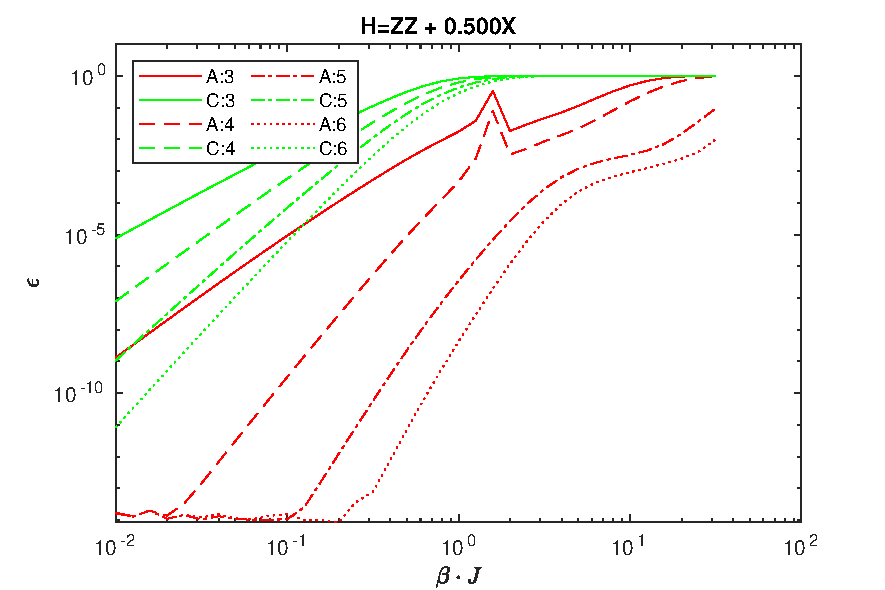
\includegraphics[scale=0.6]{Figures/1D_ising.pdf}
    \end{figure}
\end{frame}


\begin{frame}
    \begin{figure}
        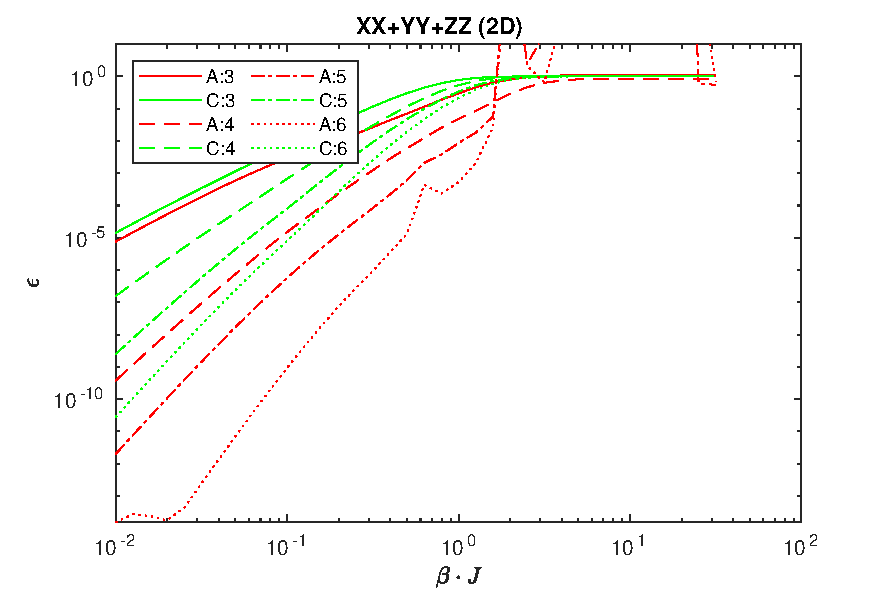
\includegraphics[scale=0.6]{Figures/1D_heis.pdf}
    \end{figure}
\end{frame}

%------------------------------------------------
%------------------------------------------------
\section{Construction 2D}
%------------------------------------------------
%------------------------------------------------

%------------------------------------------------
\subsection{ Linear blocks}
%------------------------------------------------


\begin{frame}{Construction 2D: Linear blocks}
    \begin{equation}
        \mpob{1}{ {,}  }{}{}{}{{,,}}
    \end{equation}

    \begin{equation}
        \pepob{2}{2}{{"1",,}}{{,,}}{{0,0,1,1}}  \pepob{2}{2}{{,,}}{{"1",,}}{{0,1,0,1}}
    \end{equation}



\end{frame}


\begin{frame}{Construction 2D: Linear blocks}
    \begin{equation}
        \begin{split}
            \pepob{2}{2}{{"1","1",}}{{"1","1",}}{{0,0,0,1}}  \pepob{2}{2}{{"1","1",}}{{"1","1",}}{{0,0,1,0}}\pepob{2}{2}{{"1","1",}}{{"1","1",}}{{0,1,0,0}} \pepob{2}{2}{{"1","1",}}{{"1","1",}}{{1,0,0,0}}\\
            \pepob{3}{2}{{"1","1","1","1"}}{{"1","1","1","1"}}{{0,0,0,1,1,1}} \pepob{2}{3}{{"1","1","1","1"}}{{"1","1","1","1"}}{{0,1,0,1,0,1}}
        \end{split}
    \end{equation}
\end{frame}

\begin{frame}{Construction 2D: Linear blocks}
    \begin{equation}
        \pepob{3}{2}{{"1","1","1","1"}}{{"1","1","1","1"}}{{0,0,0,1,0,1}}
    \end{equation}

    \begin{equation}
        \pepob{3}{3}{{"1","1","1","1","1","1",}}{{"1","1","1","1","1","1",}}{{1,0,1,0,0,0,1,0,1}}
    \end{equation}
\end{frame}

\begin{frame}{Construction 2D: Linear blocks}
    \begin{equation}
        \begin{split}
            \mpob{5}{ {,"1","2","2","1",}  }{}{}{}{{,,,,,}} \Rightarrow &\pepob{3}{2}{{"2","1","2","1",}}{{"1","1","1",,}}{{0,1,1,0,0,0}}\\
            &\pepob{3}{2}{{"2","1",,}}{{"1","1",,,}}{{0,0,0,0,1,1}}
        \end{split}
    \end{equation}
    And many more "linear" blocks
\end{frame}

%------------------------------------------------
\subsection{Loops}
%------------------------------------------------
\begin{frame}{Loops}


    \def \figone {{\pepob{2}{2}{{,,,,}}{{,,,,}}{{0,0,0,0}}}}
    \def \figtwo {{\pepob{2}{2}{{"$\alpha$","$\alpha$",}}{{"$\alpha$","$\alpha$",}}{{0,0,0,0}}}}

    \begin{equation}
        \figtwo
    \end{equation}

    \begin{equation}
        \pepob{3}{2}{{"$\beta$","$\beta'$","$\beta$","$\beta'$"}}{{"$\beta'$","$\alpha$","$\beta'$",,}}{{0,0,0,0,0,0}} \pepob{2}{3}{{"$\beta$","$\alpha$","$\beta$",,}}{{"$\beta'$","$\beta$","$\beta'$","$\beta'$"}}{{0,0,0,0,0,0}}
    \end{equation}

    \begin{itemize}
        \item bond dim
        \item solver: see later
    \end{itemize}

\end{frame}

\begin{frame}{Unsolved}
    \begin{equation}
        \pepob{3}{3}{{,,,,,,,,}}{{,,,,,,,,}}{{0,0,1, 0,0,0, 1,0,0,0}} \pepob{3}{3}{{,,,,,,,,}}{{,,,,,,,,}}{{1,0,0, 0,0,0, 0,0,1}}
    \end{equation}

    Easy to solve on finite lattice, dificut in thermodynamic limit...
\end{frame}


% \exp -\beta H( & \pepob{2}{2}{{,,,,}}{{,,,,}}{{0,0,0,0}})\\
%- \pepob{2}{2}{{,,,,}}{{,,,,}}{{0,0,0,0}}

%------------------------------------------------
%------------------------------------------------
\section{Solvers}
%------------------------------------------------
%------------------------------------------------



%------------------------------------------------
\subsection{Numerical considerations}
%------------------------------------------------
\begin{frame}{Numerical considerations}
    Normalisation: PEPS $O \rightarrow O/ \alpha$
    \begin{equation}
        \frac{ \exp A } { \alpha^N }  =  \exp \left(   A- N \ln{\alpha} \cdot I \right)
    \end{equation}

    Avoid large values in tensor
\end{frame}

\begin{frame}{Fast cell contraction}
    \begin{itemize}
        \item Bottleneck: find all possible contractions of virtual levels
        \item Solution: Construct sparse PEPO, contract geometry
    \end{itemize}

    \begin{figure}
        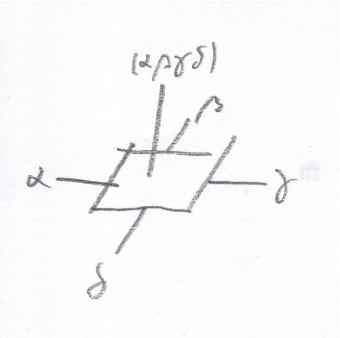
\includegraphics[scale=0.8]{Figures/pepo_contraction.pdf}
    \end{figure}
\end{frame}

%------------------------------------------------
\subsection{Problem statement}
%------------------------------------------------
\begin{frame}{Solver}
    \begin{itemize}
        \item "Linear" problems
        \item non-linear problems
    \end{itemize}
\end{frame}

%------------------------------------------------
\subsection{Linear solver}
%------------------------------------------------

\begin{frame}{Linear Solver}
    \begin{figure}
        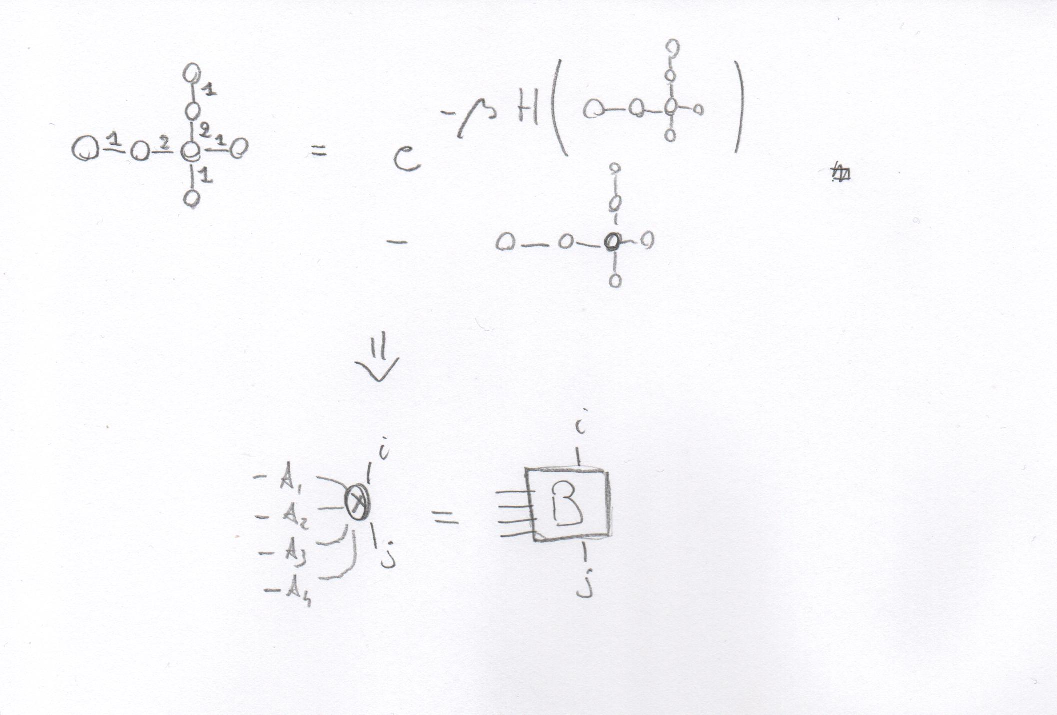
\includegraphics[scale=0.6]{Figures/linprob.pdf}
    \end{figure}
\end{frame}

\begin{frame}{Linear solver}
    \begin{itemize}
        \item types of inversion
        \item numerical stability
        \item implemented for any shape
        \item if connected -> split with SVD
    \end{itemize}

    \begin{figure}
        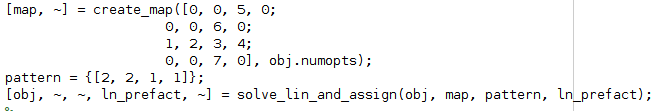
\includegraphics[scale=0.5]{Figures/mexample.png}
    \end{figure}

\end{frame}


%------------------------------------------------
\subsection{Non-linear solvers}
%------------------------------------------------
\begin{frame}{sequential linear}
    \begin{itemize}
        \item initialize randomly
        \item use linear sovler for 1 tensor
        \item fast
    \end{itemize}
\end{frame}


\begin{frame}{true non-linear solver}
    \begin{itemize}
        \item Matlab fsolve
        \item exact jocobian
        \item multiple patterns
        \item multiple maps
    \end{itemize}
\end{frame}


%------------------------------------------------
%------------------------------------------------
\section{2D Transversal Ising Model}
%------------------------------------------------
%------------------------------------------------


%------------------------------------------------
\subsection{Overview}
%------------------------------------------------
\begin{frame}{Overview}
    \begin{equation}
        \hat{H} = -J \left (  \sum_{<i j>} \sigma^x_i \sigma^x_j + \Gamma \sum_i \sigma^z_i \right )
    \end{equation}
\end{frame}

\begin{frame}{Overview}
    \begin{figure}
        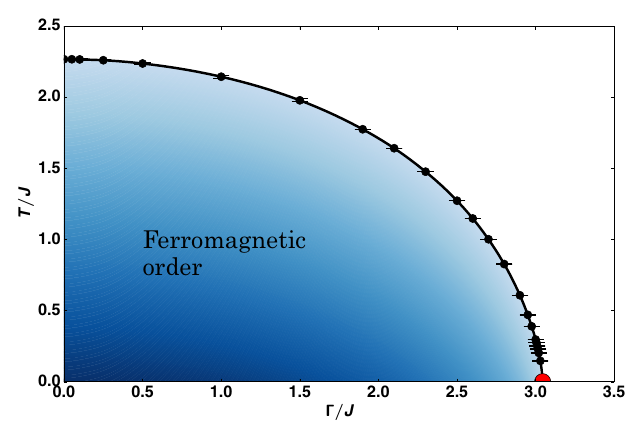
\includegraphics[scale=0.5]{Figures/2disingphase.png}
        \caption{figure taken from \cite{PhysRevB.93.155157}}
    \end{figure}
\end{frame}


%------------------------------------------------
\subsection{First results}
%------------------------------------------------
\begin{frame}{First results}
    \begin{figure}
        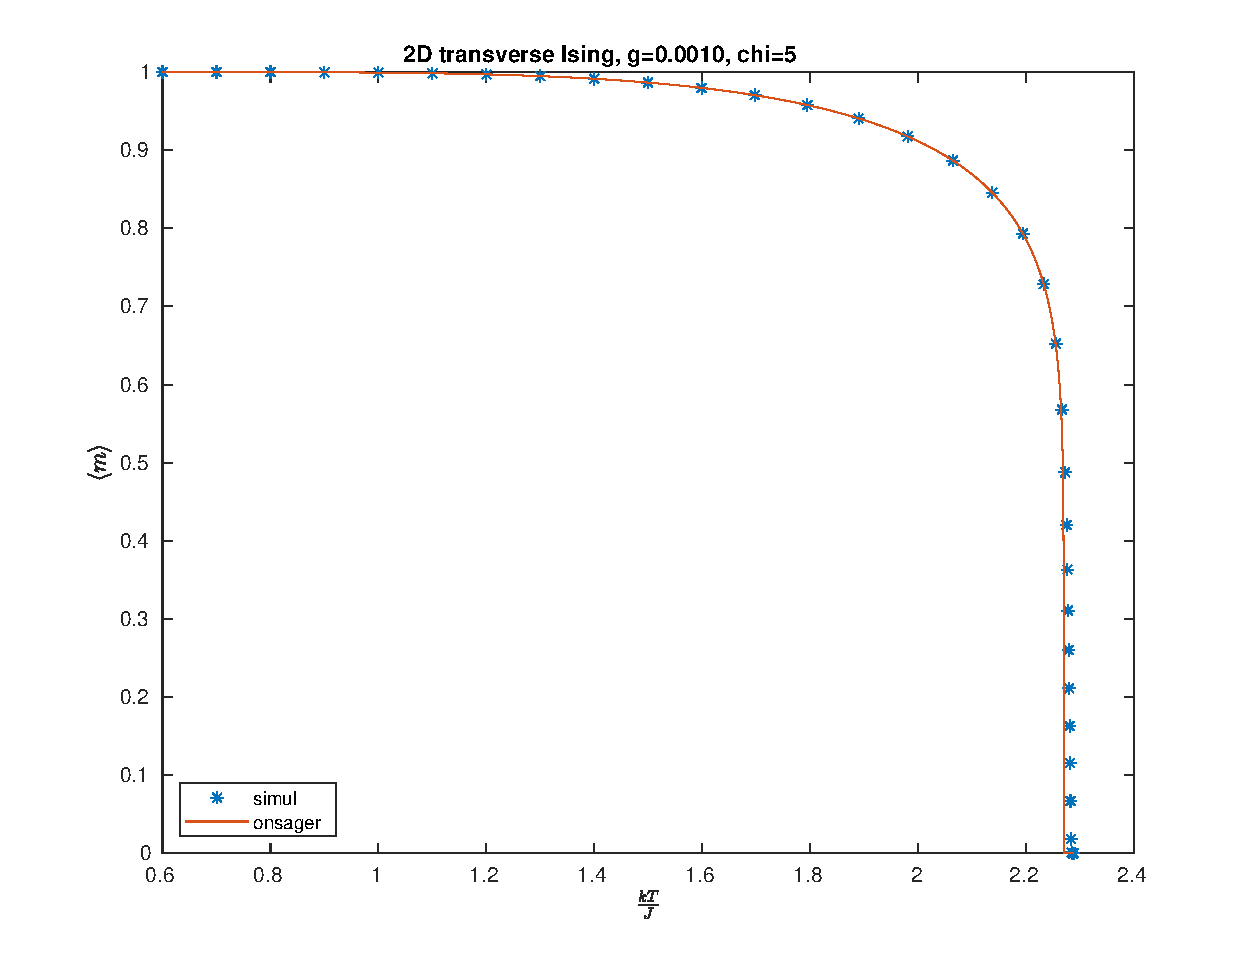
\includegraphics[scale=0.4]{Figures/g00.pdf}
    \end{figure}
\end{frame}

\begin{frame}{First results}
    \begin{figure}
        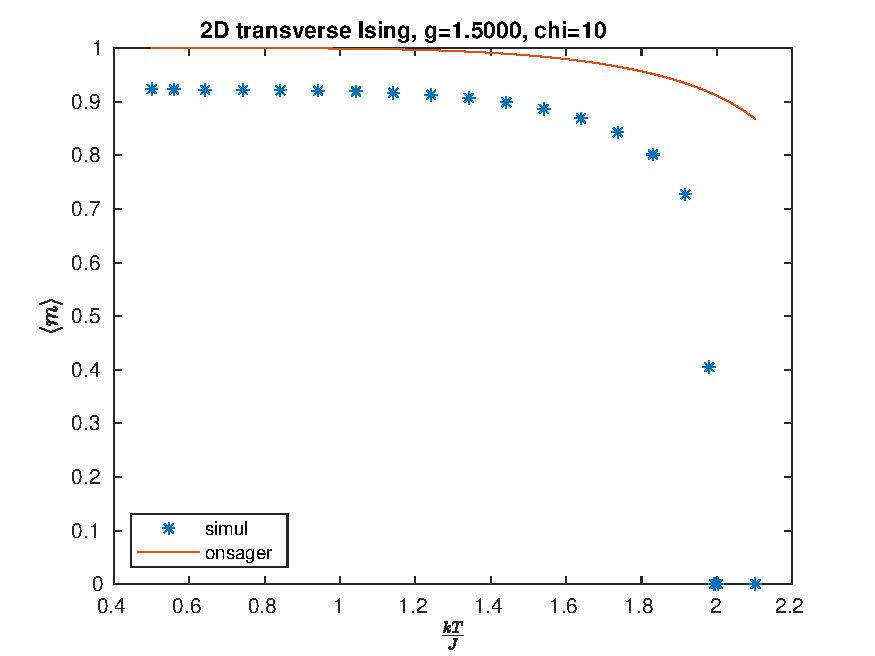
\includegraphics[scale=0.4]{Figures/g15.pdf}
    \end{figure}
\end{frame}

\begin{frame}{First results}
    \begin{figure}
        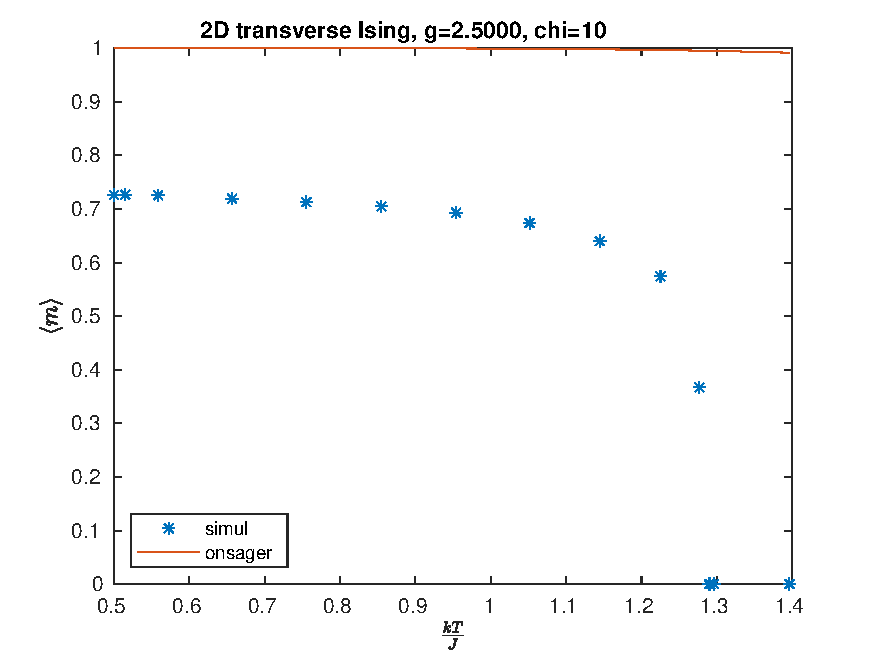
\includegraphics[scale=0.4]{Figures/g25.pdf}
    \end{figure}
\end{frame}

\begin{frame}{First results}
    \begin{figure}
        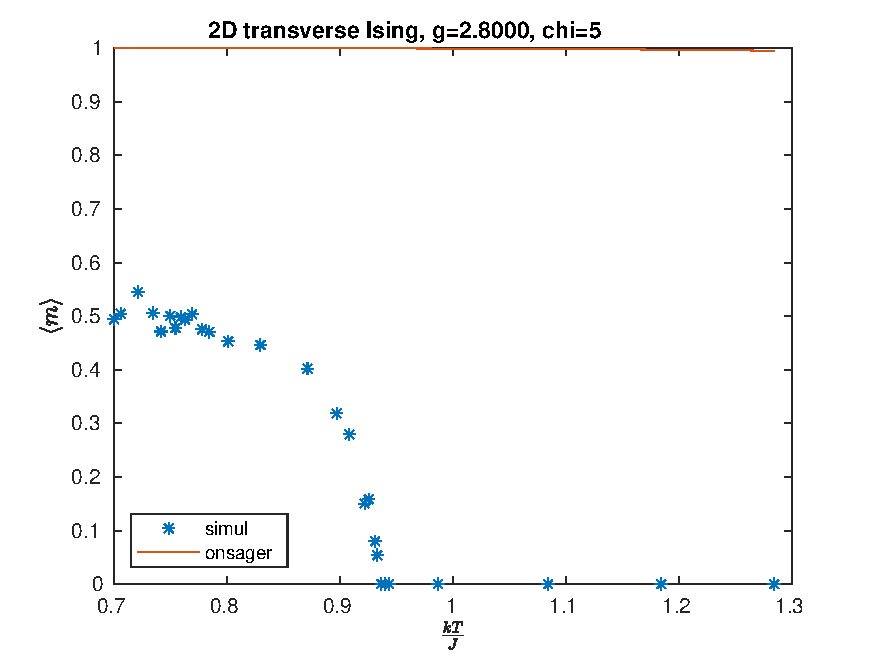
\includegraphics[scale=0.4]{Figures/g28.pdf}
    \end{figure}
\end{frame}


%------------------------------------------------
%------------------------------------------------
\section{Conclusion and outlook}
%------------------------------------------------
%------------------------------------------------
\begin{frame}{Conclusion}
    \begin{itemize}
        \item Working code for 1D and 2D
        \item General solvers
        \item Promising results in 1D and 2D
    \end{itemize}
\end{frame}


\begin{frame}{Short term}
    \begin{itemize}
        \item Accurate estimate Transversal ising quantum critical point
        \item Improve blocks for loops
        \item
    \end{itemize}
\end{frame}


\begin{frame}{Short term}
    \begin{itemize}
        \item Incorporate symmetries Hamiltonian
        \item Look at other models
        \item Generalize for other lattice geometries
        \item Generalize to 3D
    \end{itemize}
\end{frame}

\begin{frame}[allowframebreaks]
    \frametitle{References}
    \bibliographystyle{elsarticle-num}
    \bibliography{bib}
\end{frame}


\end{document}